\documentclass[a4paper,final,ngerman,english]{article} 
\usepackage[a4paper,final,pdfdisplaydoctitle,pdfauthor={My name},pdftitle={Title of my paper}]{hyperref}
\usepackage{amsmath,amsthm,amssymb,amsfonts,pgf,algorithm,algorithmic,array,multirow,fixltx2e,colortbl,tabularx,rotating,listings,stmaryrd,ifsym,marvosym}
\usepackage[ngerman]{babel} %New german orthography
\usepackage[T1]{fontenc} 
\usepackage{ucs}
\usepackage[utf8x]{inputenc}
\usepackage{lmodern} 
\usepackage{textcomp}
\usepackage{subcaption}
\usepackage{listings}
\usepackage{amsmath}
\usepackage{amssymb}
\lstset{
language=C,
tabsize=4,
showstringspaces=false
}

\pdfcompresslevel=9
%
\begin{document}
\lstset{postbreak=\space,breakindent=5pt,breaklines,basicstyle=\scriptsize,frame=trbl,label=DescriptiveLabel} %Set defaults for listings
\selectlanguage{english} %probably not necessary, just to be on the safe side
\pagestyle{headings}
%
\title{Plasma scaling study}
\author{Simon Haendeler, Severin Staudinger}
%\institute{Fakultät für Informatik, Universität Wien}
\maketitle
%
\begin{abstract}
	We are examining the scaling of the PLASMA library in case of the Cholesky Decomposition.
	We compare the runtime when using a different amount of cores and compare this to the runtime
	of LAPACK\@. To verify correctness we computed residuals. 
\end{abstract}
\section{Introduction}
In this paper we demonstrate how a driver function of PLASMA~\cite{plasma01} scales.
Therefor we decided to show this by the cholesky factorization, which is an important decomposition of symmetric positive definite matrices in the field of scientific computing.\\
To achieve this we implemented PLASMA's \textit{DPOTRF} routine and measured the processing time of its execution on two, four, eight, sixteen, 32 and 48 cores. For time measuring we used the library PAPI~\cite{papi02}.\\
All measurements were done on a system with an x86\_64 architecture, 48 CPUs, one thread per core, AMD Opteron\texttrademark{} Processor 6174 with a theoretical peak performance of 2200.00 MHz. Furthermore there are 8 NUMA nodes, which combine six cores per each node.
Since it was not easy to found out how many instructions per cycle (IPC) this particular AMD processor can handle, we assumed that it is just as high as in similiar processors of AMD. In ~\cite{amd05} it says that the number of operations which the processor can handle in one cycle is four.
In the end we compared PLASMA's \textit{DPOTRF} runtimes to the sequential cholesky decomposition implemented in LAPACK~\cite{lapack03} and calculated absolute and relative speedups.

\section{Implementation}
In order to build PLASMA we installed OpenBLAS~\cite{openblas04} and LAPACK from the latest stable releases.
Since on our system is just one thread per core we built OpenBLAS single-threaded with \textit{MAKE USE\_THREAD=0}.
To guarantee portability we decided to make a bash-script, which install every necessary library fully automatically and also auto-generate a Makefile, which compiles our \textit{main.c} programm.
This is very useful, because anybody who is interested in this PLASMA scaling study can simply run this script with \textit{bash plasma\_lapack\_blas.sh}.
After small adjustments of the generated template\_Makefile the user can compile the programm with \textit{make}.
\\
To execute the programm simply type into the terminal \textit{"./main n cores"} or \textit{"./main n l"} if you want to measure LAPACKs Cholesky Decomposition.\\ The parameter $n$ stands for the matrix size and $cores$ stands for the number of cores which are used for the computation.\\
To verify a correct execution of the test programm we used valgrind -memcheck, which found no errors.\\
Since the cholesky decomposition is only possible for symmetric positive definite we generated diagonale dominant matrices, because they are always positive definite.
\begin{lstlisting}
void generateMatrix(double *A, int n) {

	double random_number;
	srand(time(NULL));

	for (int j = 0; j < n; j++) {
		for (int i=j; i<n; i++) {
			random_number = ((double)rand() / ( (double)RAND_MAX ));
			A[i*n+j] = random_number;
			A[j*n+i] = random_number;
		}
	}

	// make positive definite
	for (int i=0; i<n; i++) {
		A[i*n+i] += n;
	}

}
\end{lstlisting}

As you can see we simply added n to the diagonal entries, so the sum of the corresponding row elements is less than n. This guarantees that matrix A is positive definite.\\
\ \\
For time measurement itself we used \textit{PAPI\_flops()}.
\begin{lstlisting}
int measure_PLASMA_dpotrf(double* A, double* L, double* work, PLASMA_enum uplo, int n, int cores) {

	error = PLASMA_Init(cores);
	if(error != PLASMA_SUCCESS){
		printf("{\"ERROR-TEXT"}\n", error, error);
		exit(1);
	}

	PAPI_flops(&rtime, &ptime, &flpops, &mflops);
	error = PLASMA_dpotrf(uplo, n, L, n);
	PAPI_flops(&rtime, &ptime, &flpops, &mflops);

	error = PLASMA_Finalize();
	if(error != PLASMA_SUCCESS){
		printf("{\"ERROR-TEXT\n", error, error);
		exit(1);
	}
	
	//these are just shortened code snippets
}
\end{lstlisting}
\ \\
To verify correctness of PLASMAs and LAPACKs decompositions we calculated residuals.
We used the one-norm. The closer the results are to zero the better they are.\\
\ \\
formular:
\(\frac{||L*L^T-A||_1}{||A||_1}\)\\


\begin{lstlisting}
double residual(double* L, double* A, double* work, int n) {

	//make L lower triangular
	for (int j=1; j<n; j++) {
		for (int i=0; i<j; i++) {
			L[j*n+i]=0;
		}
	}
	// L L^t
	PLASMA_dgemm(PlasmaNoTrans, PlasmaTrans, n, n, n, 1, L, n, L, n, 0, work, n);

	// LL^t - A
    	cblas_daxpy( n*n, -1, A, 1, work, 1 );

	double o_value = PLASMA_dlange(PlasmaOneNorm, n, n, work, n);
	double A_norm = PLASMA_dlange(PlasmaOneNorm, n, n, A, n);

	return o_value/A_norm;

}
\end{lstlisting}
Since there is no function in PLASMA, LAPACK or BLAS which can compute a matrix multiplication with two triangular matrices as an input we had to set the upper entries of the matrix L to zero.\\
In the beginning of our implementation we used here BLAS and LAPACK functions, because we don't measure execution time of the residual calculation. When testing we recognized that the residual computation takes a lot of time and so we replaced all functions with the related PLASMA ones.\\
This resulted in a far quicker execution.
\ \\
For gathering output data we coded a python-script which hashed the data. This made further processing e.g. plotting a lot easier.

\section{Evaluation}
Because the measurement was done on a shared system
we could not guarantee that our program was the only one running.
Measurement errors through context switches and alike are possible.
Each datapoint represents 5 measurements that were averaged so that small measurement errors cancel out.
Systematic error could still be present i.e.\ long running processes which affect all measurements
are still possible. Although we tried to control for those manually via htop and similar tools, we cannot exclude
those with 100\% certainty.

\begin{figure}[h!]
	\centering
	\begin{subfigure}{0.4\textwidth}
		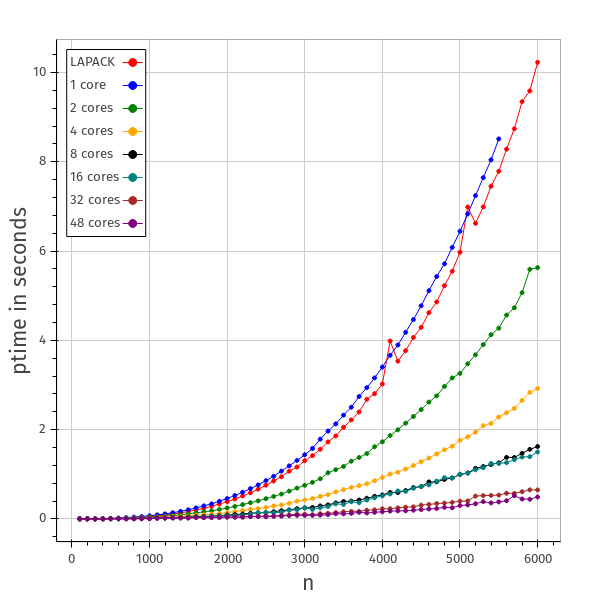
\includegraphics[width=\textwidth]{ptime}
		\caption{Process time}
\label{fig:runtime}
	\end{subfigure}
	\begin{subfigure}{0.4\textwidth}
		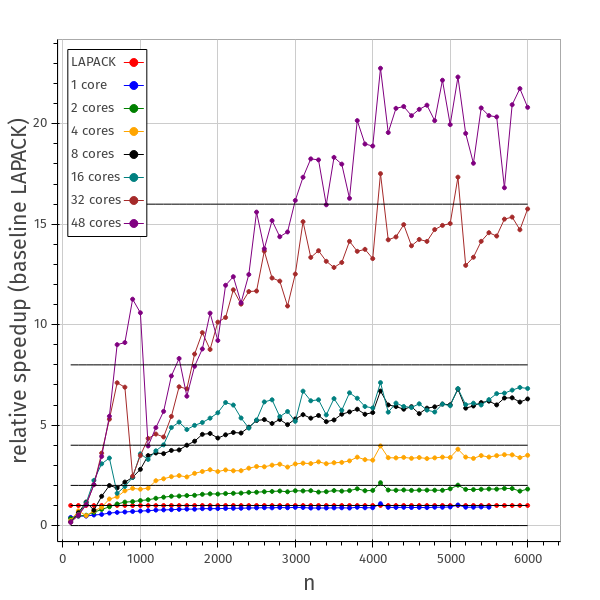
\includegraphics[width=\textwidth]{relSpeedup}
		\caption{Relative Speedup}
\label{fig:rel}
	\end{subfigure}
	\caption{Runtime of PLASMA vs LAPACK}
\end{figure}

In figure~\ref{fig:runtime}
we see the runtime of the LAPACK version and of the PLASMA version with different amount of cores/threads used.
As expected the runtime mostly increases like \(x^3\).
The single threaded PLASMA version is slightly slower than the sequential LAPACK version.
The other PLASMA versions are faster the more cores there are, at least for $n$ large enough.
The versions for 8 and 16 threads are very close together. 32 and 48 threads are also close, although
we expect that this gap should be relativly narrow.
There are bumps in the graph of the LAPACK version for \(n = 4100\) and \(n = 5100 \).

In figure~\ref{fig:rel}
we see the relative speedup for each version.
For comparison there are black lines at 2, 4, 8, 16, 32, 48 which represent the theoretical possible speedups.
We can see that the parallel versions start slower than the sequential version.
Then for relatively low $n$ each version archieves a local maxima.
For a higher thread number the $n$ is higher when the maxima is reached. 

Only 2 and 4 threads nearly reaches its theoretical performance, the higher the amount of threads,
the worse the performance relatively to the theoretical performance.

\begin{figure}[h!]
	\centering
	\begin{subfigure}{0.4\textwidth}
	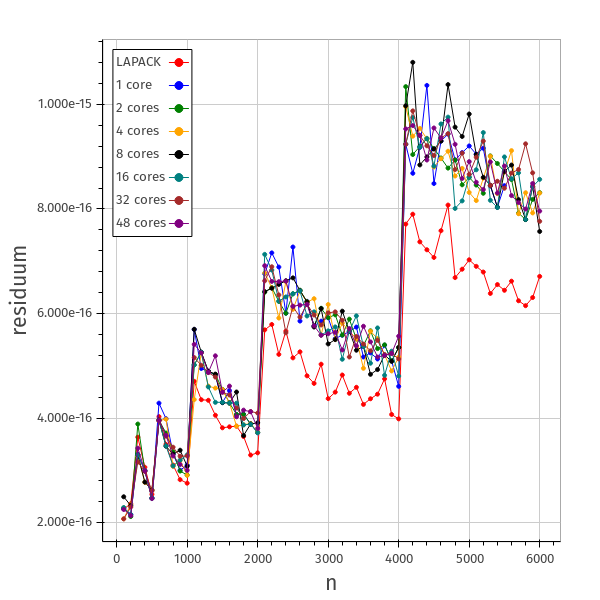
\includegraphics[width=\textwidth]{res}
	\caption{Residuum}
\label{fig:residuum}
	\end{subfigure}
	\begin{subfigure}{0.4\textwidth}
	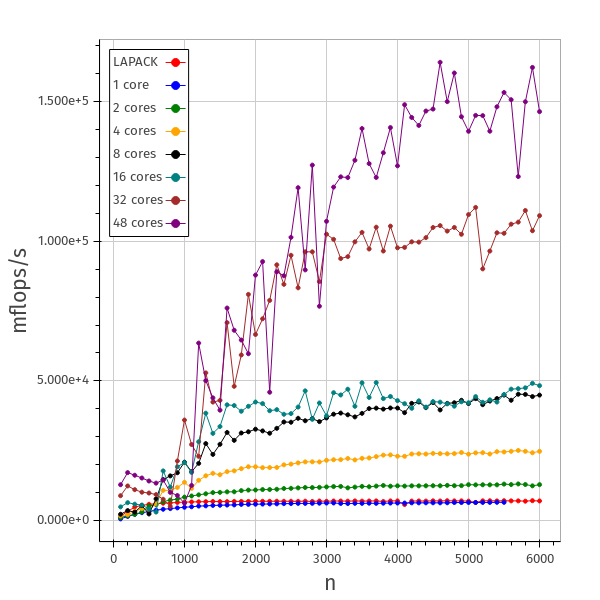
\includegraphics[width=\textwidth]{mflops}
	\caption{MFlops per second}
\label{fig:mflops}
	\end{subfigure}
	\caption{Residuum and Performance comparisons}
\end{figure}

The residuum is shown in figure~\ref{fig:residuum}.
All PLASMA versions have the same residuum behavior, but LAPACK is always a bit better.  
There are certain thresholds after which the residuual gets worse (200, 500, 1000, 2000, 4000).
After these sudden increases the residuum gets better with higher $n$.

In figure~\ref{fig:mflops} we see the Mflops per second.
We see that both LAPACK and PLASMA with one core are very similar. 

\section{Conclusions}
When looking at the runtime we can see that PLASMA scales with additional cores. 
For a lower amount of cores the scaling is very good and nearly multiplies the performance with the amount of cores.
As soon as we go higher than 8 the scaling gets worse.
The test server has 4 CPUs with each 12 cores, so when the number of cores is higher than 12 additional
overhead should come into play.
32 cores reaches the performance we would have wished for 16 cores.
This trend also goes on with 48 cores, the maximum on the system. 

LAPACK has consistently a better residuum than PLASMA.\@
This is very surprising, because LAPACK is used internally of PLASMA.\@
Maybe the merging of the subsolutions of the multiple LAPACK invocations affect the accuracy.
In that case we would expect the residuum to grow with the number of cores, which we cannot see here.
Maybe we could see this if the residuum was more stable, i.e.\ when averaging over a higher number of trails.
One could also do additional statistic analysis of the result.
But because the residuum is good enough in the PLASMA case we will not further discuss it here.

It is also surprising that the residuum gets better with higher $n$ between the jumps.
The jumppoints have a very systematic distribution, so it is likely that
LAPACK changes some parameters when around these thresholds.

For mflops we roughly get 150 Gflops.
This is \~70\% of the theoretical peak performance of 211 Gflops/s.
The numbers seems very high when compared to other publications e.g.~\cite{lawn266}.

%  
\bibliographystyle{plain} %Switches are plain,unsrt,abbrv,alpha.
\begin{footnotesize}
  \bibliography{techreport} %Publications
\end{footnotesize}

\end{document}

